\documentclass[12pt,american,czech]{article}
\usepackage[a4paper]{geometry}
\geometry{verbose,tmargin=2cm,bmargin=2cm,lmargin=2cm,rmargin=2cm,headheight=0.8cm,headsep=1cm,footskip=0.5cm}
\setcounter{secnumdepth}{3}
\usepackage{url}
\usepackage{amsmath}
\usepackage{amsthm}
\usepackage{amssymb}
\usepackage{graphicx}
\usepackage{setspace}
\usepackage{enumerate} %roman enumiration
\usepackage{threeparttable}
\usepackage{algorithmic}
\usepackage{algorithm}
\usepackage{subfigure}
\usepackage{array}
\usepackage[utf8]{inputenc} % Required for inputting international characters
\usepackage[T1]{fontenc} % Output font encoding for international characters
\usepackage{mathpazo} % Palatino font


\pagenumbering{arabic}

\makeatletter
%%%%%%%%%%%%%%%%%%%%%%%%%%%%%% Algorithms
% Define a \HEADER{Title} ... \ENDHEADER block
\newcommand{\HEADER}[1]{\ALC@it\underline{\textsc{#1}}\begin{ALC@g}}
	\newcommand{\ENDHEADER}{\end{ALC@g}}
\renewcommand*{\ALG@name}{Algoritmus}
\algsetup{indent=2em} 
\renewcommand{\algorithmiccomment}[1]{\hspace{2em}// #1} 
\makeatother

%% Use Times New Roman font for text and Belleek font for math
%% Please make sure that the 'esint' package is turned off in the
%% 'Math options' page.
\usepackage[varg]{txfonts}


%% Indent even the first paragraph in each section
\usepackage{indentfirst}

% completely avoid orphans (first lines of a new paragraph on the bottom of a page)
\clubpenalty=9500

% completely avoid widows (last lines of paragraph on a new page)
\widowpenalty=9500

% disable hyphenation of acronyms
\hyphenation{CDFA HARDI HiPPIES IKEM InterTrack MEGIDDO MIMD MPFA DICOM ASCLEPIOS MedInria}

%%---------------------------------------------------------------------

%% Print out all vectors in bold type instead of printing an arrow above them
%%\renewcommand{\vec}[1]{\boldsymbol{#1}}

% Replace standard \cite by the parenthetical variant \citep
%\renewcommand{\cite}{\citep}

\makeatother
%\pagestyle{empty} %turns off page numbering
\usepackage{babel}
\newcommand*\Laplace{\mathop{}\!\mathbin\bigtriangleup}
\newcommand*\midpoint[1]{\overline{#1}}

\begin{document}
\selectlanguage{american}
\def\documentdate{...}


\begin{titlepage} % Suppresses displaying the page number on the title page and the subsequent page counts as page 1
	\newcommand{\HRule}{\rule{\linewidth}{0.5mm}} % Defines a new command for horizontal lines, change thickness here
	\center % Centre everything on the page	
	
	\textsc{\LARGE FNSPE CTU}\\[1.5cm] % Main heading such as the name of your university/college
	\vfill
	
	\textsc{\Large Dynamic Decision Making}\\[0.5cm] % Major heading such as course name
	\textsc{\large Seminar Paper}\\[0.5cm] % Minor heading such as course title
	\HRule\\[0.4cm]
	{\huge\bfseries Minority Game}\\
	{\LARGE\bfseries From the Dynamic Decision Making Perspective}\\[0.4cm] % Title of your document
	\HRule\\[1.5cm]
	{\large\textit{Author}}\\
	Vladislav \textsc{Belov}\\
	\vfill\vfill\vfill\vfill\vfill\vfill\vfill % Position the date 3/4 down the remaining page
	{\large\today} % Date, change the \today to a set date if you want to be precise
	
	%------------------------------------------------
	%	Logo
	%------------------------------------------------
	
%	\vfill\vfill
%	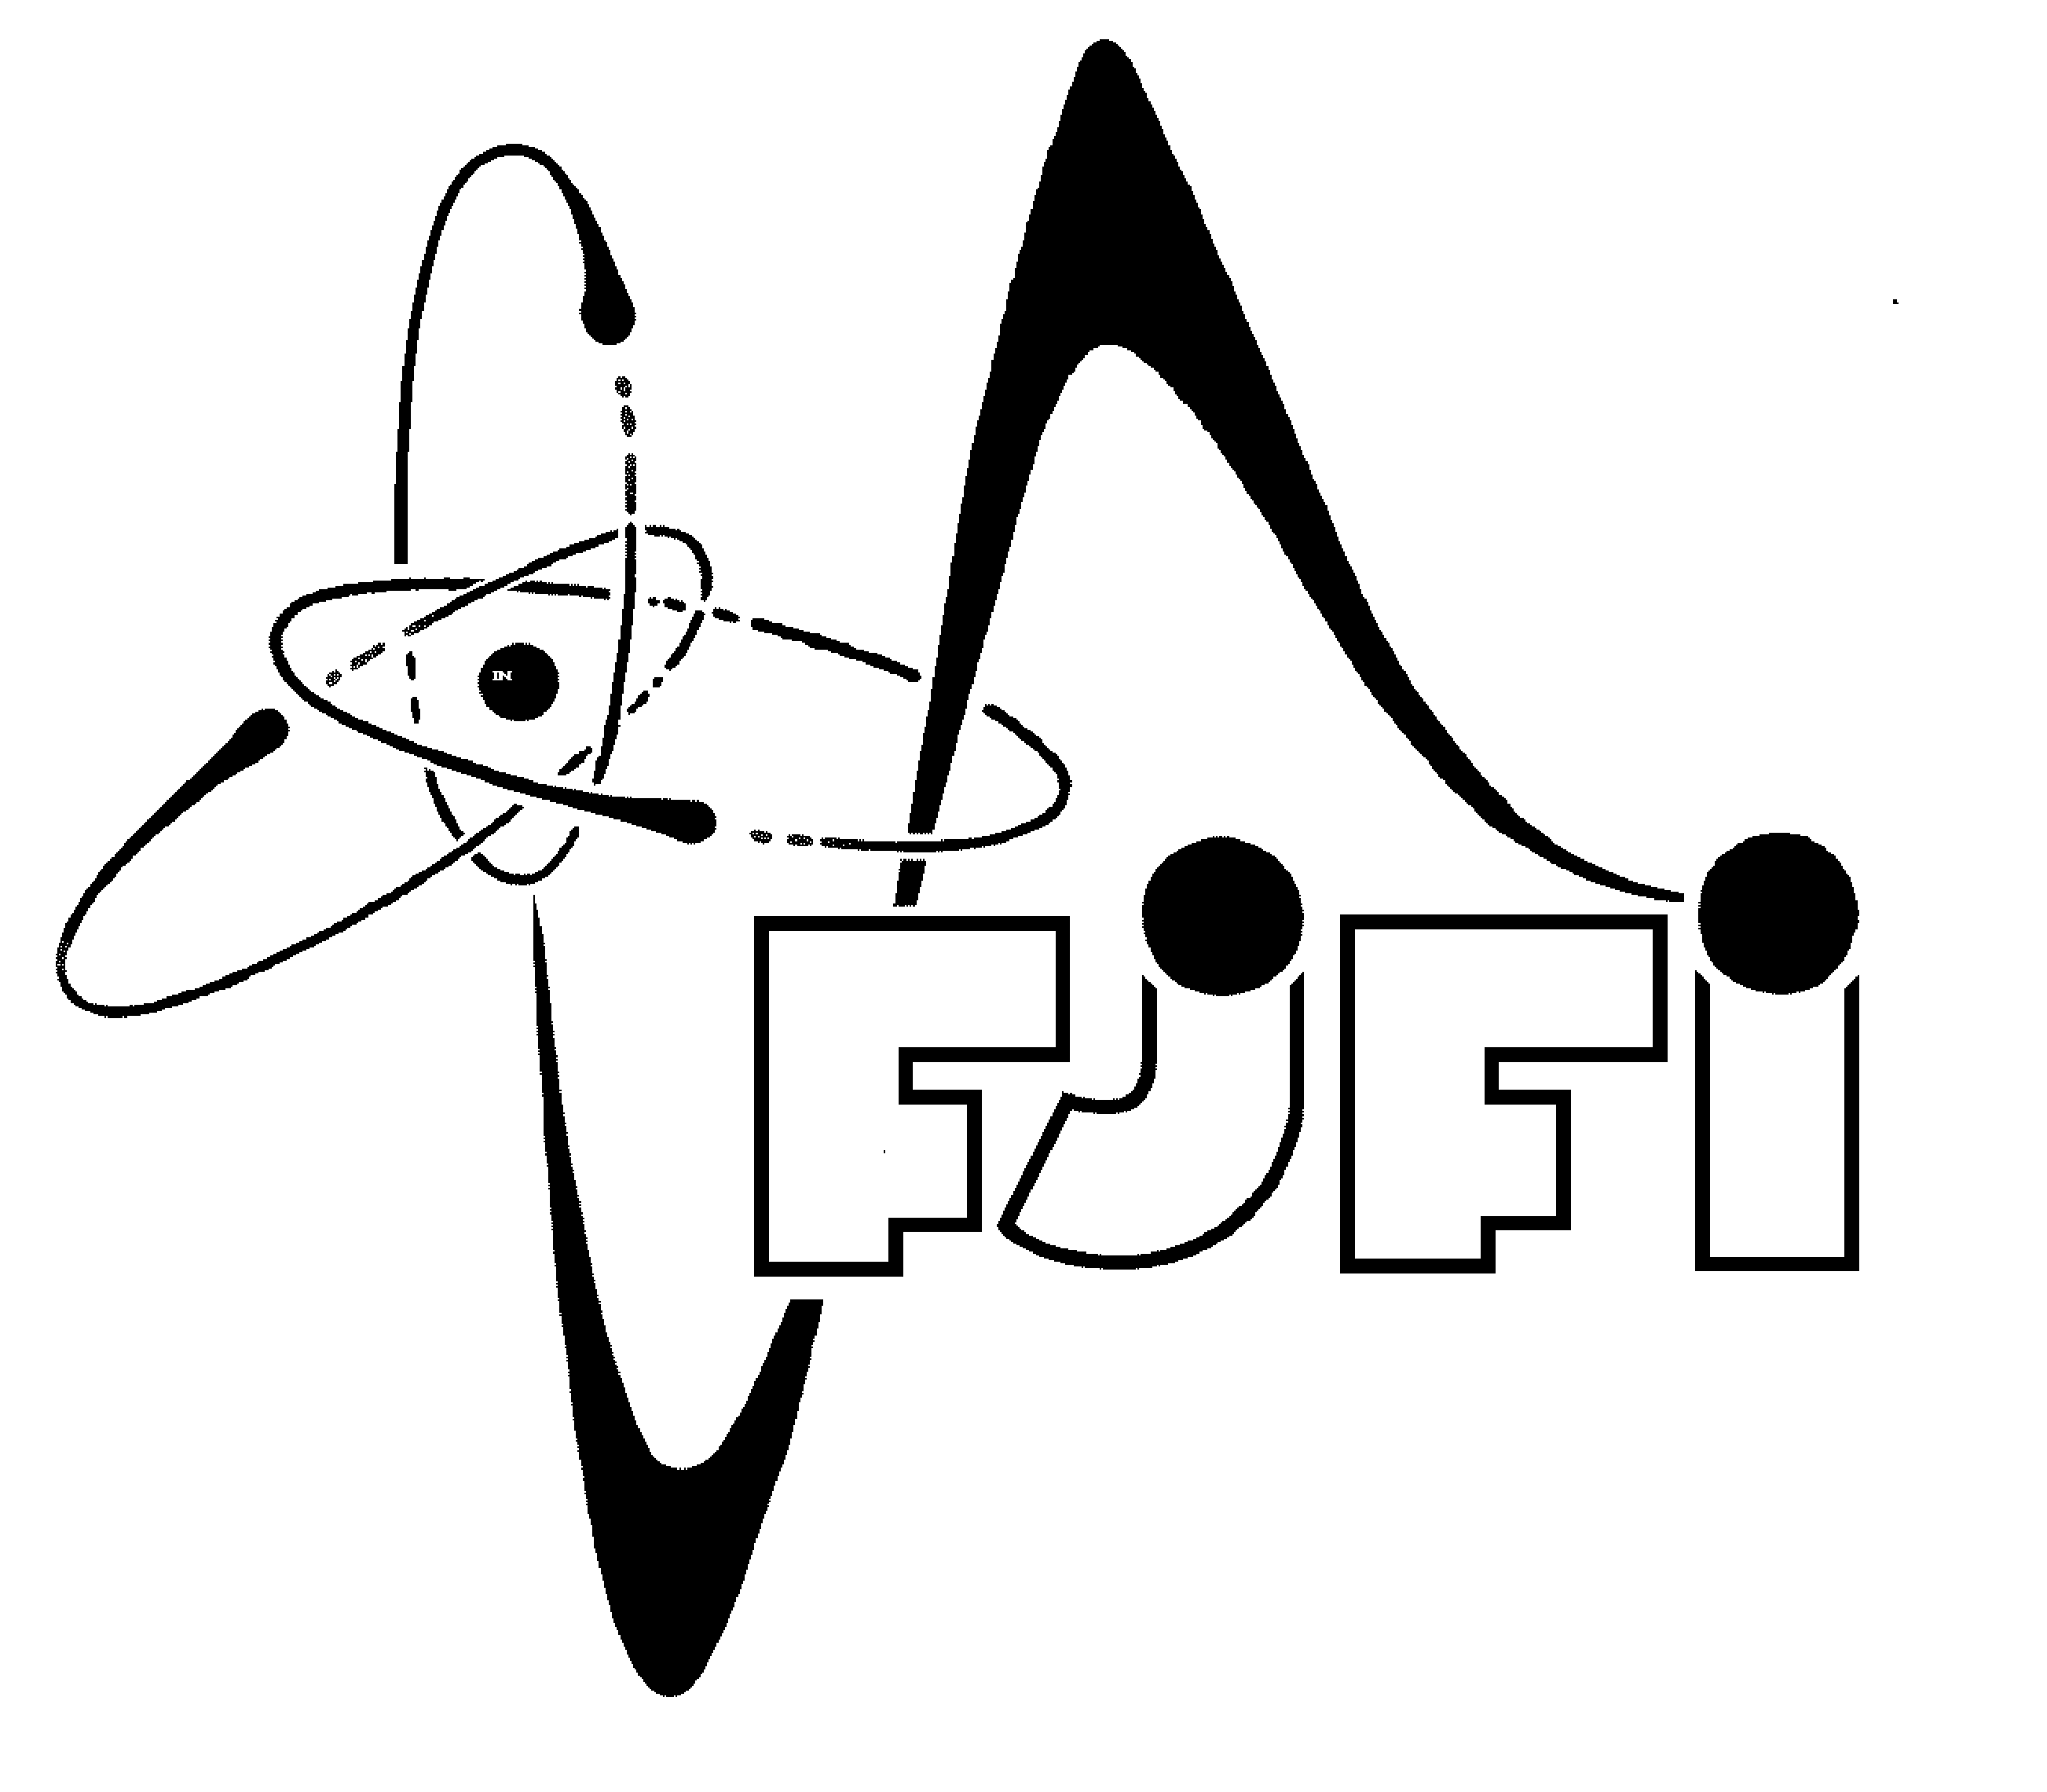
\includegraphics[width=0.2\textwidth]{Images/TITLE/fjfi}\\[1cm] % Include a department/university logo - this will require the graphicx package
%	
	%----------------------------------------------------------------------------------------
	
	\vfill % Push the date up 1/4 of the remaining page
	
\end{titlepage}

%\tableofcontents
%\newpage{}

\section{Introduction}\label{sec:introduction}

In the following seminar paper the Minority Game is going to be discussed. In the next section we will define the general mathematical model of the Minority Game. Afterwards, Q-learning and Roth-Erev learning will be introduced.

\medskip
 
The system the Minority Game describes originates from the El Farol Bar Problem which was introduced by the economist W.B. Arthur \cite{ARTHUR1994}. It goes as follows: every Thursday the population of Santa Fe has a desire to visit the bar: if more than 60 \% of people come to the bar, then it is considered to be overcrowded, so it is no fun there; if less, then the visit is pleasant and those who stayed at home are at a loss. Therefore, it can be easily seen, that the minority wins in games of El Farol Bar Problem type, that is the reason why the model has such a name. Nowadays this model is used frequently in Finance, Network Analysis, Biology, etc. \cite{CHALLET2005}

\section{Mathematical Model of the Minority Game}

Firstly, consider an odd $N=2k-1$, $k\in\{1,2,\dots\}$, number of agents participating in the game \cite{CHALLET1997,MORO2004,CHALLET2005,JOHNSON2003}. At each time step $t\in\{1,2,\dots\}$ each agent has to make a decision whether to perform an action $+1$ (e.g. go to the bar, sell an asset on the market) or $-1$ (e.g. stay at home, buy an asset on the market). Formally designated $\forall i\in\{1,2,\dots,N\}$:

\begin{equation}
a_{i}(t)=\pm 1.
\end{equation}

In order to study game dynamics a special parameter called \textit{total action} was introduced: 

\begin{equation}
A(t)=\sum_{i=1}^{N}a_{i}(t), \forall t\in\{1,2,\dots\},
\end{equation}

\noindent
which is basically the sum of actions performed by every agent at a given game round.

\medskip

After each game round the outcome is disclosed to each of the agents: as soon as the round is finished, everyone gets to know what the winning action was. This action $W(t+1)$ ($t+1$ is used to specify, that this information is available at a time step $t+1$) is determined by a simple rule:

\begin{itemize}
\item $A(t)>0$ $\implies$ the action $-1$ was victorious, $W(t+1)=-1$;
\item $A(t)<0$ $\implies$ the action $+1$ was victorious, $W(t+1)=1$;
\item $A(t)=0$ will never occur due to oddness of $N$.
\end{itemize} 

\noindent
In other words, $W(t+1) = -\text{sign}\big(A(t)\big)$.

\medskip

Minority  Game is a system of agents with bounded memory: each agent remembers $m\in\{1,2,\dots\}$ recent game outcomes. This \textit{recent history} can be represented two different ways:

\begin{itemize}
	\item As an $m$-tuple of most recent game outcomes: $\bar{\mu}(t)=(W(t-m+1),W(t-m+2),\dots,W(t))$;
	\item As a single decimal number $\mu(t)$ with binary representation equal to $\bar{\mu}(t)$.\footnote{E.g.: let $m=3$, then for $\bar{\mu}(t)=(-1,-1,1)$ its decimal representation (obtained by applying the transformation $-1\rightarrow 0$) is $\mu(t)=1$, because $001_{2}=1_{10}$.}
\end{itemize} 

\noindent
It can be easily seen, that in total $2^{m}$ possible recent histories exist, therefore, $\mu(t)\in\{0,1,\dots,2^{m}-1\}$.

\medskip

At the beginning of the game each agent gets a fixed number of strategies. For any fixed $m$ a \textit{strategy} is a mapping $\pi:(0,1,\dots,2^m-1)\mapsto\{-1,1\}^{2^{m}}$ (all possible outcomes are mapped to respective actions, e.g. see Table~\ref{tab:strategy_table_example}). The construction of such mapping implies, that agents are able to get from $1$ to $2^{2^{m}}$ strategies. The set of strategies available to agent $i\in\{1,2,\dots,N\}$ will be called \textit{agent's strategic portfolio} and denoted as $\mathcal{P}_{i}$. The action/decision of agent $i$ with respect to recent history $\mu(t)$ using the strategy $\pi$ will be denoted as $\pi_{i}(\mu(t))$, e.g. if agent $i$ uses the strategy from the Tab.~\ref{tab:strategy_table_example} when recent history is $101$, then $\pi_{i}(5)= -1$.

\begin{table}
	\centering
	\begin{tabular}{|c|c||c|}
		\hline
		Recent History, $\bar{\mu}(t)$ & $\mu(t)$ & Action/Decision \\
		\hline
		\hline 
		$0 0 0$ & 0 & $-1$ \\ 
		$0 0 1$ & 1 & $+1$ \\ 
		$0 1 0$ & 2 & $+1$ \\ 
		$0 1 1$ & 3 & $-1$ \\ 
		$1 0 0$ & 4 & $+1$ \\ 
		$1 0 1$ & 5 & $-1$ \\ 
		$1 1 0$ & 6 & $+1$ \\ 
		$1 1 1$ & 7 & $+1$ \\
		\hline
	\end{tabular} 
	\caption{Strategy example for $m=3$.} 
	\label{tab:strategy_table_example}
\end{table}

\medskip

Now the question arises: how to model the process of decision making? In the following section we will discuss the original standard learning mechanism, Q-learning and Roth-Erev learning.

\section{Learning in the Minority Game}

To begin, we will try to describe the Minority Game in a more general way. It is a complex system where agents need memory to make an optimal decision and not all relevant portions of the environment can be observed - we are dealing with partially observable, stochastic, sequential, dynamic, discrete, multi-agent environment. Depending on the learning mechanism, the set of states can be defined differently (compare subsections \ref{subsec:original} and \ref{subsec:q}). 

\medskip

Let $(\mathcal{S},\mathcal{A},\mathcal{T},\mathcal{R})$ be a Markov Decision Process where $\mathcal{S}$ is a state space, $\mathcal{A}$ is a set of possible actions, $\mathcal{T}$ is a transition model, $\mathcal{R}$ is a reward model. Obviously, both the transition model $\mathcal{T}$ and the reward model $\mathcal{R}$ are not available for agents in the Minority Game, therefore, agents have to learn "along the way".

\medskip

This paper is focused on introduction and brief comparison of different learning mechanisms for the Minority Game and what is their impact on the performance of a single agent. Let agent $i\in\{1,2,\dots,N\}$ has won $w_{i}(t)$ rounds and lost $l_{i}(t)$ rounds, $w_{i}(t)+l_{i}(t)=t$, then its \textit{performance} or \textit{profit} at a time $t$ is defined as:

\begin{equation}
p_{i}(t) = w_{i}(t)-l_{i}(t).
\end{equation}

\subsection{Standard Learning Mechanism}\label{subsec:original}

For any fixed $m$ let $\mathcal{S}=\big\{\mu(t):\mu(t)\in\{0,1,\dots,2^{m}-1\}\big\}$ and $\mathcal{A}=\cup_{i}\mathcal{A}_i$ where $\mathcal{A}_i=\{$choose strategy $\pi$ : $\pi\in\mathcal{P}_{i}$ $\}$, $\forall i\in\{1,2\dots,N\}$. The original learning mechanism is based on giving strategies scores which will be updated as the game progresses, in other words, if the strategy was successful during the recent round, then its score is increased, and vice versa. The update rule of the score for strategy $\pi$ denoted as $R^{\,\pi}$ is defined as follows:

\begin{equation} \label{eq:mg_score_upd}
R^{\,\pi}(t+1) = R^{\,\pi}(t)-\pi\big(\mu(t)\big)\cdot g\big(A(t)\big)
\end{equation}

\noindent
where $g$ is any odd function with respect to total action $A(t)$.\footnote{Here for simplicity $g(\cdot)=\text{sign}(\cdot)$.} 

\medskip

At each game round agents choose the best scoring strategy from the ones available for them:

\begin{equation}
\pi_{i}^{\text{opt}} = \arg \max_{\pi\in\mathcal{P}_{i}} R(t),\,\forall i\in\{1,2\dots,N\}.
\end{equation}

The strategy score can in some sense be interpreted as the reward function, but such an assumption is a bit misleading. 

\subsection{Q-learning Mechanism}\label{subsec:q}

The Q-learning approach is based on the update of Q-function which is an expected total reward from taking action $a\in\mathcal{A}$ at state $s\in\mathcal{S}$. Its update rule is defined as:

\begin{equation}
Q_{i}(s,a)\leftarrow(1-\alpha)\cdot Q_{i}(s,a)+\alpha\cdot\big(r(s)+\gamma\cdot\max_{a'}Q_{i}(s',a')\big)
\end{equation}

\noindent
where $s'$ is the next state, $\alpha$ is a learning parameter, $\gamma$ is a discount factor and $r$ is an immediate reward at state $s$.

Let $\mathcal{S}=\{\pi: \pi \text{ is a strategy}\}$, the set of possible actions will be defined as $\mathcal{A}=\cup_{i}\mathcal{A}_i$ where $\mathcal{A}_i=\{$switch from using the strategy $\pi$ to $\tilde{\pi}$ : $\pi,\tilde{\pi}\in\mathcal{P}_{i}\}$, $\forall i\in\{1,2\dots,N\}$. Now Q-learning may be applied to the Minority Game \cite{ANDRECUT2002}. The action-state function denoted as $Q_{i,\pi,\tilde{\pi}}$ has the following meaning:

\begin{itemize}
\item If $\pi=\tilde{\pi}$, then the agent $i$ will not change his current strategy to another one;
\item If $\pi\neq\tilde{\pi}$, then the agent $i$ will switch from strategy $\pi$ to $\tilde{\pi}$.
\end{itemize}

Agent $i\in\{1,2,\dots,N\}$ will choose its optimal strategy given by the following equation at each time step by the $\varepsilon$-greedy rule:\footnote{Strategy $\pi_{i}^{\text{opt}}$ will be chosen with probability $1-\varepsilon$, otherwise the other strategy is chosen randomly from the rest of agent's strategic portfolio.}

\begin{equation}
\pi_{i}^{\text{opt}} = \arg \max_{\tilde{\pi}\in\mathcal{P}_{i}} Q_{i,\pi,\tilde{\pi}},\,\forall i\in\{1,2\dots,N\}.
\end{equation}


Action-state function update rule which has to be evaluated at each game round will take form:

\begin{equation}
Q_{i,\pi,\tilde{\pi}}\leftarrow (1-\alpha)\cdot Q_{i,\pi,\tilde{\pi}}+\alpha\cdot\big(r(\tilde{\pi})+\gamma\cdot\max_{\pi'}Q_{i,\pi,\pi'}\big)
\end{equation}

\noindent
where after using the strategy $\tilde{\pi}$ agent's immediate reward is $r(\tilde{\pi})=-\tilde{\pi}(\mu(t))\cdot A(t)$. That means, if $\tilde{\pi}$ was successful, then the reward is $\arrowvert A(t)\arrowvert$,  and $-\arrowvert A(t)\arrowvert$ in the opposite case.

\subsection{Roth-Erev Learning Mechanism}\label{subsec:rerl}

Roth-Erev reinforcement learning is completely different from the techniques discussed in subsections \ref{subsec:original} and \ref{subsec:q}. Here agents are not given any strategies according to the original model, decision making is based on \textit{propensities} to take specific actions and propensity update rule. Although the state space $\mathcal{S}$ can be defined the same way as in the subsection \ref{subsec:original}, the set of possible actions is now $\mathcal{A}=\{-1,+1\}$ and the learning mechanism is as follows \cite{WHITEHEAD2008}:

\begin{itemize}

		\item Agent $i\in\{1,2,\dots,N\}$ has a propensity $q_{i}^{\,a}(t)$ to play action $a$, $\forall a\in\mathcal{A}$. Propensities are required to meet the condition $q>0$ and they have to stay positive;\footnote{That can be achieved by defining a positive payoff function.}
		\item Let $(y_{i}(t), 1-y_{i}(t))$ represent agent's strategy at time $t$ which means, that he will take action $-1$ with probability $y_{i}(t)$, hence, the action $+1$ will be taken with probability $1-y_{i}(t)$. These probabilities are defined by a simple relation:
		
\begin{equation}
y_{i}(t)=Pr(\mathit{a}=+1)=\frac{q_{i}^{\mathit{+1}}(t)}{q_{i}^{+1}(t)+q_{i}^{-1}(t)}.
\end{equation}

		It is simple to deduce, that $Pr(\mathit{a}=-1)=1-y_{i}(t)$.
		
		\item Propensity is updated only if the taken action was successful:\footnote{In the original text \cite{WHITEHEAD2008} the update is given as some general function. The following update was proposed to perform simulations.}
		
\begin{equation}
q_{i}^{\mathit{a}}(t+1) \leftarrow q_{i}^{\mathit{a}}(t) + \frac{|A(t)|}{N}.
\end{equation}
\end{itemize}

\section{Simulations}

Based on the learning techniques introduced in the previous section a number of simulations were performed. Game parameters were set to $N=101$, $m=7$, $s=5$ and $t_{\text{max}}=1000$. During each of the simulations at a time $t_{0}=250$ the agent with the worst performance was chosen and its profit dynamics throughout the whole game was displayed (see Fig.~\ref{fig:figure_1}, \ref{fig:figure_3}, \ref{fig:figure_5}). The general descending trend can be explained with the fact, that majority always loses, however for some initial parameters (e.g. $m=7$, $s=2$) a slowly ascending or fluctuating trend may be observed.

\medskip

During simulations depicted in Fig.~\ref{fig:figure_3} and \ref{fig:figure_5} the standard learning mechanism for the tracked agent was turned off at a time $t_{0}=250$ and changed with Q-learning and Roth-Erev learning respectively. 

\section{Conclusion}

In this seminar paper the Minority Game model was introduced. In Sec. 3 we discussed different learning mechanisms for it. Simulations have shown, that Q-learning and Roth-Erev learning provide the chosen agent with a significant improvement in comparison with standard learning method. This implies, that further studies of their impact are needed.

\newpage{}

\begin{figure}[ht!]
\centering
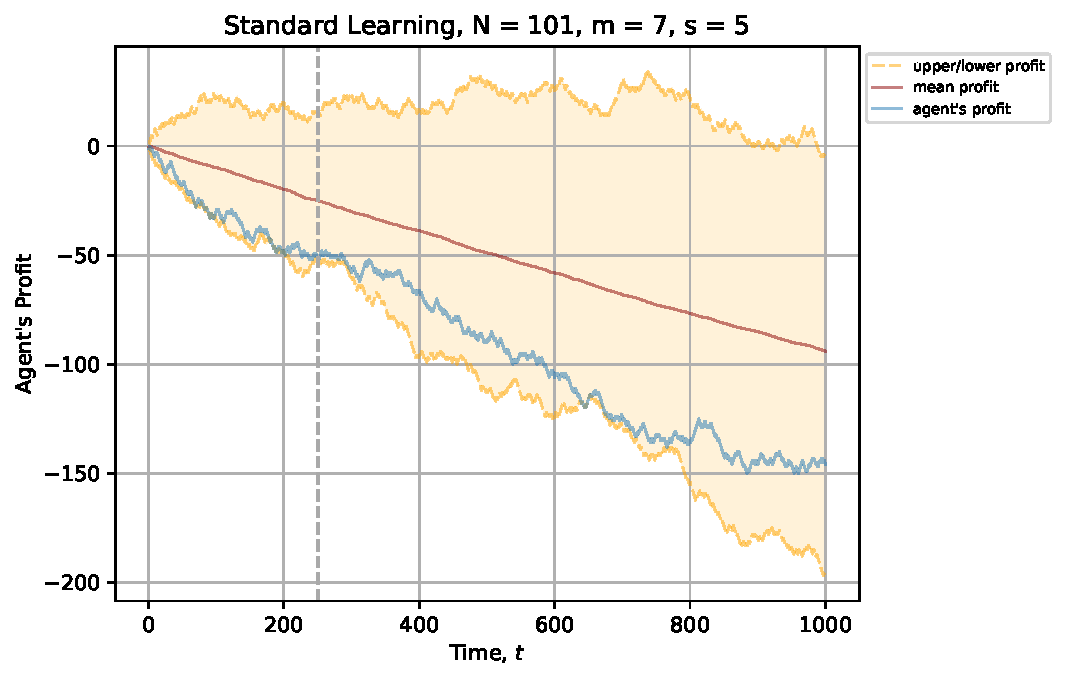
\includegraphics[width=0.8\linewidth]{Images/figure_4}
\caption{Performance of agent with standard learning mechanism.}
\label{fig:figure_1}
\end{figure}

\begin{figure}[ht!]
\centering
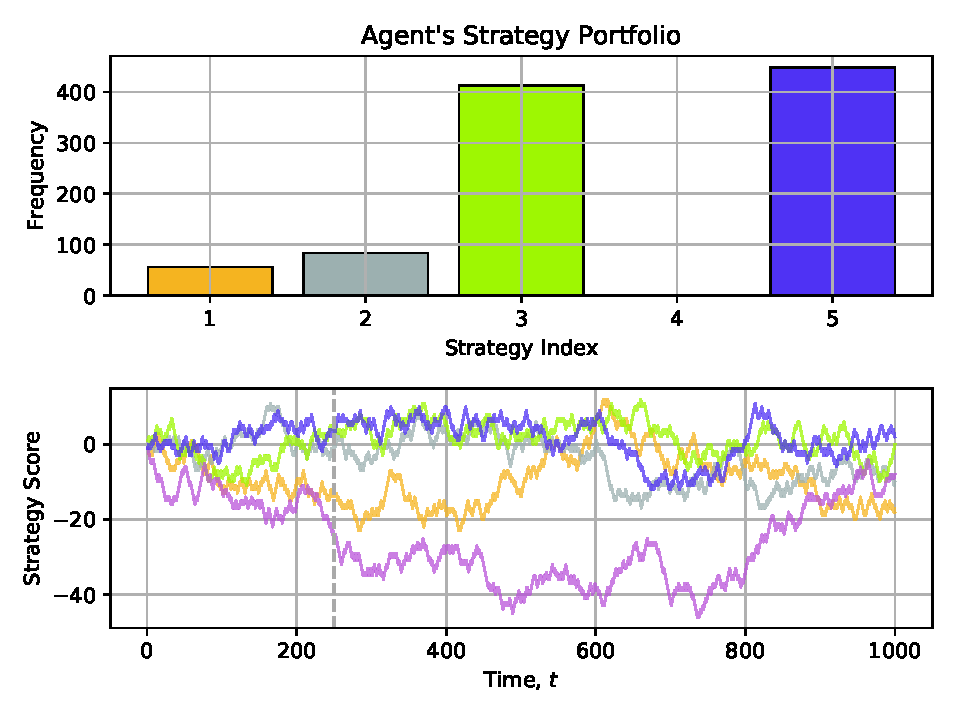
\includegraphics[width=0.7\linewidth]{Images/figure_5}
\caption{Strategy Portfolio dynamics of agent with standard learning mechanism.}
\label{fig:figure_2}
\end{figure}

\newpage{}

\begin{figure}[ht!]
\centering
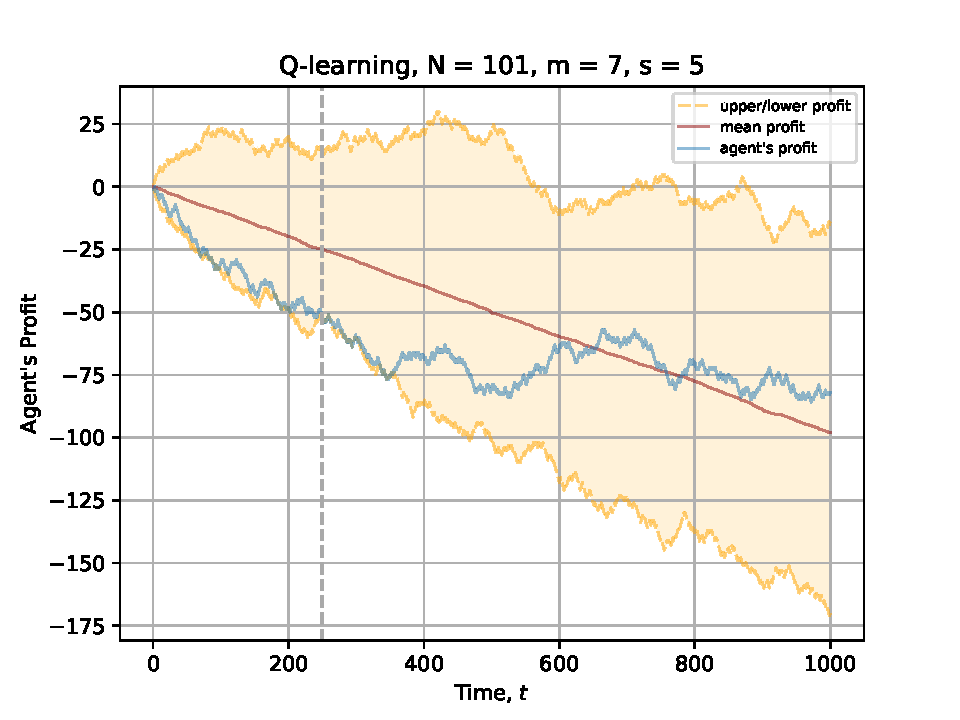
\includegraphics[width=0.8\linewidth]{Images/figure_2}
\caption{Performance of agent with Q-learning mechanism (standard learning process was switched off for it at $t_{0}=250$), $\alpha=\tfrac{1}{2^{m}}$, $\gamma=0.75$, $\varepsilon=\tfrac{250}{t}$ where $t\in\{251,252,\dots,1000\}$.}
\label{fig:figure_3}
\end{figure}

\begin{figure}[ht!]
\centering
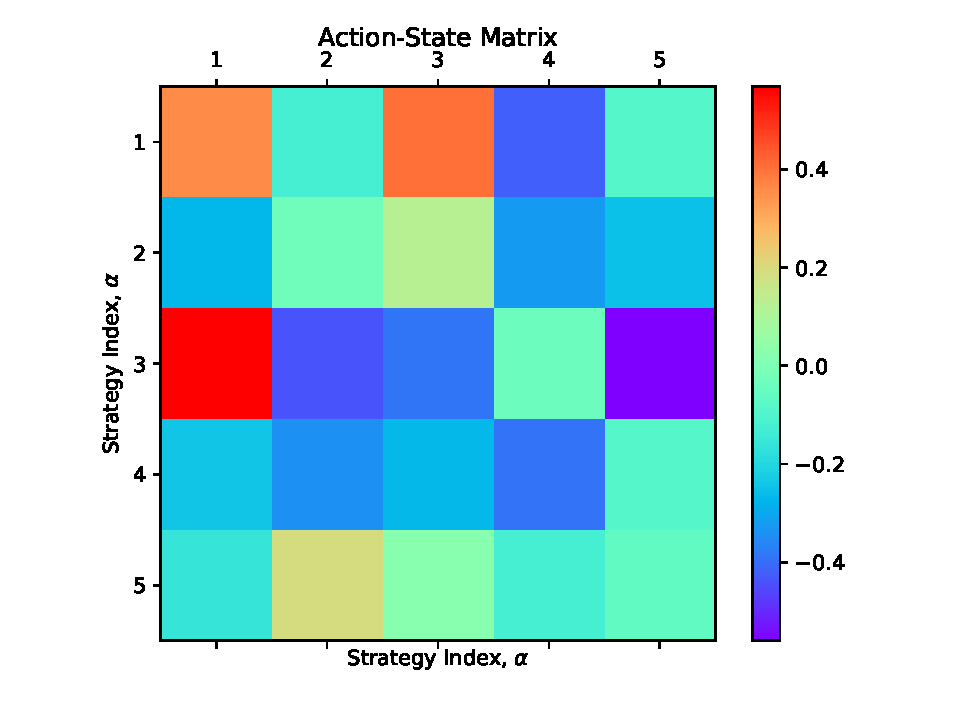
\includegraphics[width=0.8\linewidth]{Images/figure_3}
\caption{Action-state function visualization for agent with Q-learning mechanism.}
\label{fig:figure_4}
\end{figure}

\newpage{}

\begin{figure}[ht!]
\centering
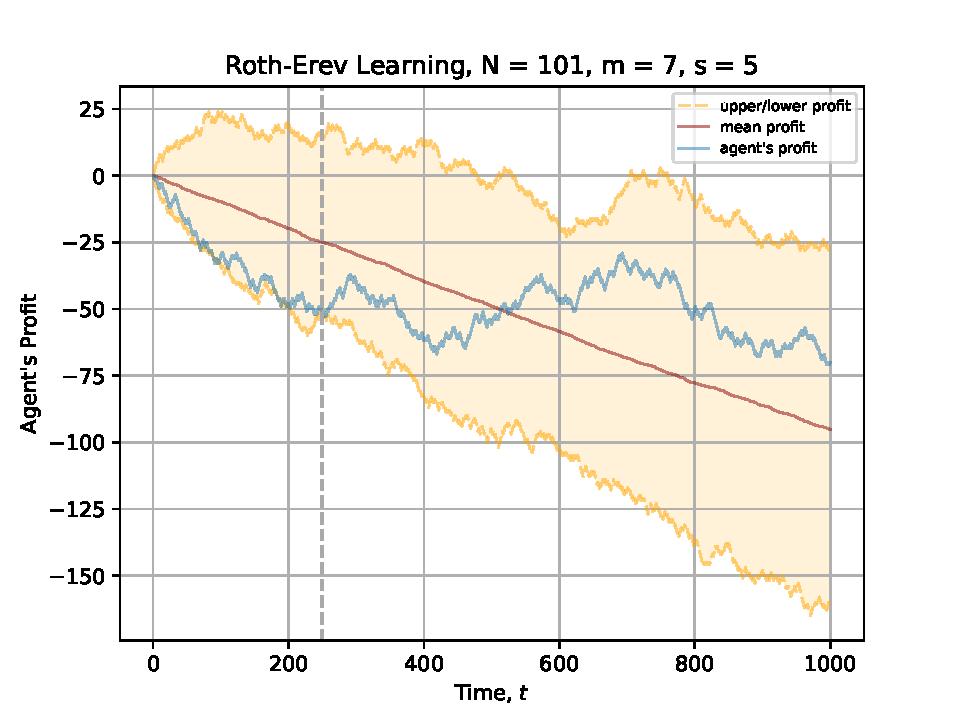
\includegraphics[width=0.8\linewidth]{Images/figure_1}
\caption{Action-state function visualization for agent with Roth-Erev learning mechanism (standard learning process was switched off for it at $t_{0}=250$).}
\label{fig:figure_5}
\end{figure}


\newpage{}

\bibliography{bib/Whitehead2008,bib/Andrecut2002,bib/Arthur1994,bib/Challet1997,bib/Johnson2003,bib/Minority_Games,bib/Moro2004}

%\bibliographystyle{plain}
\bibliographystyle{alpha}

\end{document}
